\section{Auswertung}
\label{sec:Auswertung}

\subsection{Vorbereitung}\label{subsec:Vorbereitung}
Um die Messungen auswerten zu können, muss zunächst das Eigenträgheitsmoment $I_{D}$ und die Winkelrichtgröße $D$ berechnet werden.

Mit (\ref{eq:drehmoment}) und (\ref{eq:drehmomentwinkel}) ergibt sich:
\begin{equation}
D = \frac{\lvert F \rvert \lvert r \rvert \sin{\vartheta}}{\varphi} \stackrel{F,r > 0}{=} \frac{F r \sin{\vartheta}}{\varphi} 
\stackrel{\vartheta = \frac{\pi}{2}}{=} \frac{F \cdot r}{\varphi}
\end{equation}

In Tabelle (\ref{tab:Winkelrichtgröße}) sind die entsprechenden Messwerte und die berechneten Winkelrichtgrößen.

\begin{table}
\centering
\caption{Messdaten zu Winkelrichtgröße, $r = 20 \unit{\centi\meter}$}
\label{tab:Winkelrichtgröße}
\begin{tabular}{c c c}
  \toprule
  $\varphi / °$  &  $F / \unit\newton$ & $D / \unit{\newton\meter}$ \\
  \midrule
              20 &        0.022 &     0.012605 \\
              30 &        0.054 &     0.020626 \\
              40 &        0.077 &     0.022059 \\
              50 &        0.092 &     0.021085 \\
              60 &        0.120 &     0.022918 \\
              70 &        0.144 &     0.023573 \\
              80 &        0.162 &     0.023205 \\
              90 &        0.188 &     0.023937 \\
             100 &        0.190 &     0.021772 \\
             110 &        0.200 &     0.020835 \\
             120 &        0.230 &     0.021963 \\
  \bottomrule
\end{tabular}
\end{table}

Es ergibt sich der Mittelwert:
\begin{align*}
  D_{mittel} = D  & = 0.021325364366313267 \pm 0.002952928161464375 \unit{\newton\meter}\\
  \implies D &  = 0.021 \pm 0.00295 \unit{\newton\meter}
\end{align*}

Um das Eigenträgheitsmoment zu bestimmen wird nach (\ref{eq:Tumgestellt}) I berechnet.
Dafür wird die Umlaufzeit gemessen, wobei der Stab mit zwei bekannten Massen an den Seiten ausgelenkt wird.
Dabei ist der Radius genau bestimmt.
Die Daten sind in Tabelle (\ref{tab:Eigenträgheitsmoment}) aufgetragen:

\begin{table}
  \centering
  \caption{Messdaten zum Eigenträgheitsmoment $I_{D}$}
  \label{tab:Eigenträgheitsmoment}
  \begin{tabular}{c c c c}
    \toprule
    $r / \unit\meter$  &  $T / \unit\second$ & $r^2 / (\unit\meter^2)$  & $T^2 / (\unit\second)^2$\\
    \midrule
      0.050   & 2.750   & 0.003   &  7.562  \\
      0.075   & 3.100   & 0.006   &  9.610  \\
      0.100   & 3.800   & 0.010   & 14.440  \\
      0.125   & 4.100   & 0.016   & 16.810  \\
      0.150   & 4.750   & 0.022   & 22.562  \\
      0.175   & 5.300   & 0.031   & 28.090  \\
      0.200   & 5.800   & 0.040   & 33.640  \\
      0.225   & 6.600   & 0.051   & 43.560  \\
      0.250   & 7.150   & 0.062   & 51.123  \\
      0.275   & 7.800   & 0.076   & 60.840  \\
    \bottomrule
    \end{tabular}
\end{table}

Aus diesen Daten können wir jetzt das Eigenträgheitsmoment bestimmen.
Dafür brauchen wir zunächst noch die Formeln für einen Zylinder.
Dieses lässt sich mit rechnerisch bestimmen, hier sei nur die Formel angegeben:
\begin{equation*}
  I_{\text{Zyl}} = \frac{m \cdot R^2} {2}
\end{equation*}

Mit dem Satz von Steiner (\ref{eq:SatzvSteiner}) ergibt sich:
\begin{equation} \label{eq:IZyl}
  I_{\text{Zyl}} = I_{D} + m_{\text{Zyl}}  \left( \frac{3 r^2 + h^2}{6} \right)
\end{equation}

Setzt man nun $I_{\text{Zyl}}$ in Gleichtung (\ref{eq:Tumgestellt}) ein und stellt um, erhält man folgende Gleichung:

\begin{equation}
  T^2 = \frac{4 \pi^2}{D} \cdot \left( ma^2 + I_{\text{Zyl}} \right) \stackrel{(\ref{eq:IZyl})}{=} 
  \frac{4 \pi^2}{D} \left( ma^2 + I_{D} + m_{\text{Zyl}}  \left( \frac{3 r^2 + h^2}{6} \right) \right)
\end{equation}

Nun erhält man durch lineare Regression eine Ausgleichsgerade der Form $y = a \cdot x + b$ mit den Parametern
$a = 724.885 ± 10.115$ und $b = 5.945 ± 0.400$. Damit ergibt sich der Plot in Abbildung (\ref{fig:Lineareregression}).
Nun wird durch Koeffizientenvergleich a und b in (\ref{eq:IZyl}) erkannt und eingesetzt.
Es ergibt sich:
\begin{align} \label{var:aundb}
  a & = \frac{4 \pi^2 m}{D} & b & = \frac{4 \pi^2}{D} m_{\text{Zyl}}  \left(I_{D} + \frac{3 r^2 + h^2}{6} \right)
\end{align}

\begin{figure}[H]
  \caption{Regressionsgerade des Eigenträgheitsmomentes}
  \centering
  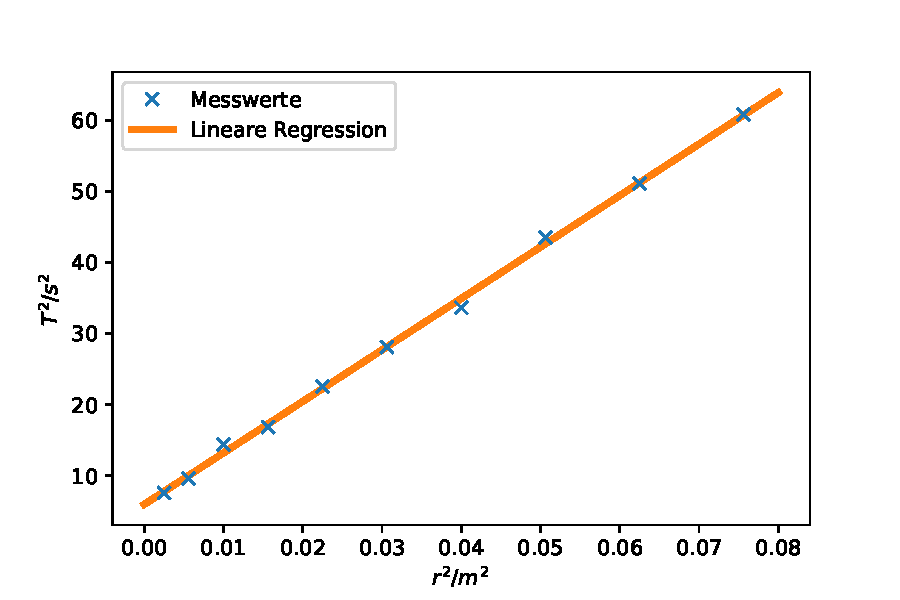
\includegraphics{pictures/Lineare Regression.pdf}
  \label{fig:Lineareregression}
\end{figure}

Stellt man nun (\ref{eq:IZyl}) nach $I_{D}$ um, gilt:
\begin{equation} \label{eq:idgauß}  % Ist diese Gleichung überhaupt richtig? Überprüfen wenn Zeit
  \begin{split}
  I_{D} {} &= I_{\text{Zyl}} - m_{\text{Zyl}}  \left( \frac{3 r^2 + h^2}{6} \right) \\
    &\stackrel{\ref{var:aundb}}{=} \frac{b \cdot D}{4 \cdot \pi^2} - m_{\text{Zyl}}  \left( \frac{3 r^2 + h^2}{6} \right)
  \end{split}
\end{equation}

Mit (\ref{fehler:gauß}) ergibt sich  für $\increment I_{D}$:

\begin{equation*}
  \increment I_{D} = \sqrt{\left(\frac{b}{4 \pi^2} \cdot  \increment D\right)^2 + \left(\frac{D}{4 \pi^2} \cdot  \increment b\right)^2}
\end{equation*}

%%%%%%%%%%%%%%%%%%%%%%%%%%%%%%%%%%%%
%%%%%%%%%%%%%%%%%%%%%%%%%%%%%%%%%%%%
%%%%%%%%%%%%%%%%%%%%%%%%%%%%%%%%%%%% Muss noch errechnet werden
%%%%%%%%%%%%%%%%%%%%%%%%%%%%%%%%%%%%

Damit lässt sich der Fehler für das Eigenträgheitsmoment angeben. Es gilt also:
\begin{equation*}
  I_{D} =  \unit{\kilo\gram\meter\squared}
\end{equation*}

Eigenträgheitsmoment vernachlässigbar?
%%%%%%%%%%%%%%%%%%%%%%%%%%%%%%%%%%%%
%%%%%%%%%%%%%%%%%%%%%%%%%%%%%%%%%%%%
%%%%%%%%%%%%%%%%%%%%%%%%%%%%%%%%%%%%
%%%%%%%%%%%%%%%%%%%%%%%%%%%%%%%%%%%%

\subsection{Trägheitsmomente von Kugel und Zylinder}
\label{sec:KugelundZylinder}

\subsubsection*{Der Zylinder}
Der betrachtete Zylinder hat folgende Maße: $m_1 = 0.3678 \unit{\kilo\gram}, d_1 = 0.0983 \unit{\meter}$
Damit errechnet sich der Theoriewert des Trägheitsmomentes:

\begin{align*}
  I_{\text{Zyl, theo}} &= 4.4425 10^{-4} \unit{\kilo\gram\meter\squared}
\end{align*}

Die experimentellen Werte sind in Tabelle (\ref{tab:SchwingungsdauerZylinder}) zu finden.

\begin{table}
  \centering
  \caption{Messung der Schwingungsdauer des Zylinders}
  \label{tab:SchwingungsdauerZylinder}
  \begin{tabular}{c c}
    \toprule
     Messung &  $T / \unit\second$ \\
    \midrule
              1 &        0.800 \\
              2 &        0.750 \\
              3 &        0.760 \\
              4 &        0.720 \\
              5 &        0.750 \\
              6 &        0.740 \\
              7 &        0.740 \\
              8 &        0.790 \\
              9 &        0.750 \\
             10 &        0.780 \\
    \bottomrule
  \end{tabular}
\end{table}

Damit lässt sich die Schwingungsdauer angeben:
\begin{equation*}
  T_{Zyl} = (0.758 \pm 0.02357) \unit{\second}
\end{equation*}


Damit ist das Trägheitsmoment $I_{\text{Zyl}}$ kann nun angegeben werden.
Der Fehler berechnet sich nach (\ref{eq:idgauß}). Es folgt:

%%%%%%%%%%%%%%%%%%%%%%%%%%%%%%%%%%%%
%%%%%%%%%%%%%%%%%%%%%%%%%%%%%%%%%%%%
%%%%%%%%%%%%%%%%%%%%%%%%%%%%%%%%%%%% Muss noch errechnet werden
%%%%%%%%%%%%%%%%%%%%%%%%%%%%%%%%%%%%

\begin{equation*}
  I_{\text{Zyl}} = 
\end{equation*}

%%%%%%%%%%%%%%%%%%%%%%%%%%%%%%%%%%%%
%%%%%%%%%%%%%%%%%%%%%%%%%%%%%%%%%%%%
%%%%%%%%%%%%%%%%%%%%%%%%%%%%%%%%%%%%
%%%%%%%%%%%%%%%%%%%%%%%%%%%%%%%%%%%%

\subsubsection*{Die Kugel}

Die betrachtete Kugel hat die folgenden Eigenschaften: $m_2 = 1.1716\unit{\kilo\gram}$ und $d = 14.645\unit{\centi\meter}$.
Die Formel für das Trägheitsmoment einer Kugel wird auch hier nur angegeben:
\begin{equation*}
  I_{\text{K}} = \frac{2}{5} m r^2
\end{equation*}
Mit den Werten bedeutet das:
\begin{equation*}
  I_{\text{K, theo}} = 1.0051 \cdot 10^{-2} \unit{\kilo\gram\meter\squared}
\end{equation*}

\begin{table}[H]
  \centering
  \caption{Messung der Schwingungsdauer der Kugel}
  \label{tab:SchwingungsdauerKugel}
  \begin{tabular}{c c}
    \toprule
    Messung &  $T / \unit\second$ \\
    \midrule
              1 &        1.770 \\
              2 &        1.900 \\
              3 &        1.850 \\
              4 &        1.800 \\
              5 &        1.800 \\
              6 &        1.800 \\
              7 &        1.900 \\
              8 &        1.850 \\
              9 &        1.880 \\
             10 &        1.870 \\
    \bottomrule
    \end{tabular}
\end{table}

Damit ergibt sich aus Mittelwert und Standartabweichung für $T_{Kug}$:
\begin{equation*}
  T_{Kug} = (1.842 \pm 0.044) \unit\second
\end{equation*}

Woraus das Trägheitsmoment $I_{\text{Kug}}$ folgt:

%%%%%%%%%%%%%%%%%%%%%%%%%%%%%%%%%%%%
%%%%%%%%%%%%%%%%%%%%%%%%%%%%%%%%%%%%
%%%%%%%%%%%%%%%%%%%%%%%%%%%%%%%%%%%%
%%%%%%%%%%%%%%%%%%%%%%%%%%%%%%%%%%%%


\begin{equation*}
  I_{\text{Kug}} = 
\end{equation*}

%%%%%%%%%%%%%%%%%%%%%%%%%%%%%%%%%%%%
%%%%%%%%%%%%%%%%%%%%%%%%%%%%%%%%%%%%
%%%%%%%%%%%%%%%%%%%%%%%%%%%%%%%%%%%%
%%%%%%%%%%%%%%%%%%%%%%%%%%%%%%%%%%%%


\subsection{Trägheitsmoment der Puppe}

\subsubsection{Abmessungen}

\begin{table}
  \centering
  \caption{Abmessungen der Puppe}
  \label{tab:Abmessungen}
  \begin{tabular}{llll}
    \toprule
    Bein (14,33 cm) & - & Arm (13,02 cm) & - \\
    \midrule
               ober &      unter &           ober &      unter \\
               1.54 &       1.64 &            1.3 &       1.24 \\
               1.64 &       1.72 &           1.31 &       1.37 \\
               1.73 &       1.42 &            1.4 &       1.42 \\
               1.84 &       1.41 &           1.24 &        1.3 \\
                1.8 &        1.3 &           1.22 &        1.2 \\
    \bottomrule
    \end{tabular}\\

    \begin{tabular}{llr}
      \toprule
      Körper (9,81 cm) & - &  Kopf (4,71 cm) \\
      \midrule
                  ober &      unter &             - \\
                  3.96 &       3.33 &            2.83 \\
                  4.24 &       5.43 &            2.97 \\
                   4.3 &        3.5 &            2.73 \\
                  3.94 &        3.3 &            2.60 \\
                  3.25 &       3.17 &            2.25 \\
      \bottomrule
      \end{tabular}
\end{table}

Die Puppe hat die folgende Masse: $m_{\text{Puppe}} = 0.1079\unit{\kilo\gram}$.
Die Maße der Gliedmaßen der Puppe sind in Tabelle (\ref{tab:Abmessungen}) aufgetragen.
Diese Werte werden gemittelt, um der die Gliedmaßen durch Zylinder zu approximieren (siehe Tabelle (\ref{tab:MittelwertGlieder})).

\begin{table}
  \centering
  \caption{Mittelwerte der Glieder}
  \label{tab:MittelwertGlieder}
  \begin{tabular}{rrrrrrrr}
    \toprule
       & $d_{\text{Bein}} / \unit\meter$ &     - &     $d_{\text{Arm}} / \unit\meter$ &     - &    $d_{\text{Körper}} /  \unit\meter$ &     - &    $d_{\text{Kopf}} /  \unit\meter$\\
    \midrule
     & ober & unter & ober & unter& ober & unter & \\
    Mittelwert: & 0.017 & 0.015 & 0.013 & 0.013 & 0.039 & 0.037 & 0.027 \\
    Standartabweichung:  &0.001 & 0.002 & 0.001 & 0.001 & 0.004 & 0.008 & 0.002 \\
    \bottomrule
    \end{tabular}
\end{table}

Im folgenden wird das Volumen der Puppe errechnet.
Dazu wird das Volumen der einzenen Zylinder berchnet.
Das Zylindervolumen ist gegeben durch:
\begin{equation*}
  V_{\text{Zyl}} = \pi r^2 h
\end{equation*}
Ebenfalls benötigt wird das Kugelvolumen, um den Kopf zu approximieren:
\begin{equation*}
  V_{\text{Kug}} = \frac{4}{3} \pi r^3
\end{equation*}

Um den Fehler anzugeben, benötigen wir noch die Gauß'sche Fehlerfortpflanzung (\ref{fehler:gauß}):

\begin{equation}
  \increment V_{\text{Ges}} = \sqrt{(\increment V_{\text{Körper}})^2 + 4 \cdot (\increment V_{\text{Arm}})^2 
    + 4 \cdot (\increment V_{\text{Bein}})^2 + (\increment V_{\text{Kopf}})^2}
\end{equation}

wobei die einzelnen Volumina durch 
\begin{align*}
  \increment V_{\text{Zyl}} &= \sqrt{4 \pi^2 \cdot r^2 \cdots h^2 \cdot (\increment r)^2} & 
  \increment V_{\text{Kug}} &= \sqrt{16 \pi^2 \cdot r^4 \cdot (\increment r)^2}
\end{align*}

Damit lassen sich die Volumina der einzelnen Körperteile angeben (Tabelle (\ref{tab:VolGlieder})):

\begin{table}[H]
  \centering
  \caption{Volumen der Körperteile}
  \label{tab:VolGlieder}
  \begin{tabular}{rrrrrrr}
    \toprule
    & Oberschenkel &     Unterschenkel &     Oberarm &     Unterarm &    Oberkörper &     Bauch \\
    \midrule
    $V / \unit{\milli\cubic\meter}$  & 13.164012 & 10.102287 & 6.849035 & 6.976654 & 47.793662 & 43.246845 \\
    $\increment V / \unit{\milli\cubic\meter}$  &  1.675321 &  2.110987 & 0.668167 & 0.864282 &  9.056683 & 19.592513 \\
    \bottomrule
    \end{tabular}
\end{table}